\documentclass{beamer}

\usepackage[italicdiff]{physics}
\usepackage{hyperref}
\usepackage{url}
\usepackage{bm}


\newcommand{\dbar}{d\hspace*{-0.08em}\bar{}\hspace*{0.1em}}

\newenvironment{itemframe}[1]{\begin{frame}{#1}\begin{itemize}}   {\end{itemize}\end{frame}}

% Changes style of actual slides
\usetheme{Dresden}
% Changes color of slides
\usecolortheme{spruce}
% removes controls at bottom right side
\usenavigationsymbolstemplate{}

% for figures
\graphicspath{ {./figs/} }

\title{Probability and Information Theory}
\author{Michael Cardiff}
\subtitle{PHYS 163a \ 09/16 Prep Work}

\begin{document}

\begin{frame}
  \titlepage
\end{frame}

\section{Coin Probability}
\begin{frame}{What does it mean to have Probability 1/2?}
  \begin{itemize}
  \item Probability of a single heads is $\frac12$
  \item We have two total outcomes
  \item One of them is heads
  \item The other is tails
  \item Unbiased means we are telling the truth, there are \textit{only} 2 options and the chance of each is equal.
  \end{itemize}
\end{frame}
\begin{frame}{What is the Probability of 6 Heads}
  \begin{itemize}
  \item Each coin flip's result is independent of the previous results
  \item So each flip has a $\frac12$ chance of being heads
  \item This means a total of 2 options per flip
  \item Total of $2\times2\times2\times2\times2\times2=2^6$ options
  \item Only one option is all heads, so there is a $\frac1{2^6}$ chance
  \end{itemize}
\end{frame}
\section{PDF? What is that?}
\begin{frame}{What is a PDF?}
  \begin{itemize}
  \item Stands for Probability \textbf{Density} Function
  \item Know about mass density: mass per volume
  \item Density in general, total quantity per some element
  \item Hence pdf = Probability per unit length
  \end{itemize}
\end{frame}

\begin{frame}{How is a pdf Related to the Probability we Descibed?}
  \begin{itemize}
  \item How to get mass from mass density?
    \begin{itemize}
    \item Take all volume elements of mass
    \item Multiply by the density
    \item Add all those together
    \end{itemize}
  \item This sounds like integrating
  \item To get probability from pdf:
    \begin{itemize}
    \item Take elements of whatever we are taking the probability per unit of
    \item Multiply by density
    \item Add together
    \item a.k.a Integrate it!
    \end{itemize}
  \end{itemize}
\end{frame}
\begin{frame}{In Terms of an Equation?}
  \begin{itemize}
  \item The probability of something happening at all should be 100\%
  \item This means we need a definite integral:
    \begin{equation}
      P(a,b)=\int_a^b\rho(X)\dd{X}
    \end{equation}
  \item Probability of the event characterized by the interval $(a,b)$ happening
  \end{itemize}
\end{frame}
\begin{frame}{Expected Value?}
  \begin{itemize}
  \item Expected Value is equivalent to a mean in discrete probability (like rolling a die)
  \item When we roll a dice a lot of times, add up what we rolled and divided by the number of rolls, what number do we get?
  \item We perform this by multiplying the 'value' of each possibility by the probability that we get it. 
  \item For a pdf this would be the $X$ in the formula, so to get an expected value we perform the following integral:
    \begin{equation}
      \ev{X}=\int X\rho(X)\dd{X}
    \end{equation}
  \item This is done over the entire range of the distribution
  \end{itemize}
\end{frame}
\begin{frame}{An Example}
  \begin{columns}
    \begin{column}{0.5\textwidth}
      \begin{itemize}
      \item Instead of a discrete score, a pdf describes a continuous value
      \item Example: Height
      \item Height is a continuous value
      \item Expected value of height = Average height of a person
      \end{itemize}
    \end{column}

    \begin{column}{0.5\textwidth}
      \begin{figure}[H]
        \centering
        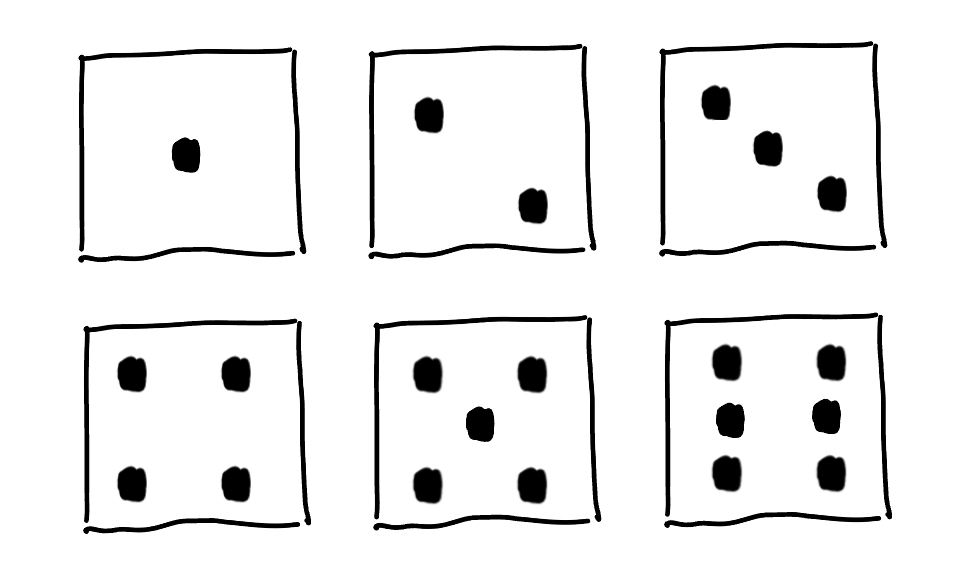
\includegraphics[width=3.5cm]{dice.jpg}
        \caption{Dice: Discrete Values}
      \end{figure}
      \begin{figure}[H]
        \centering
        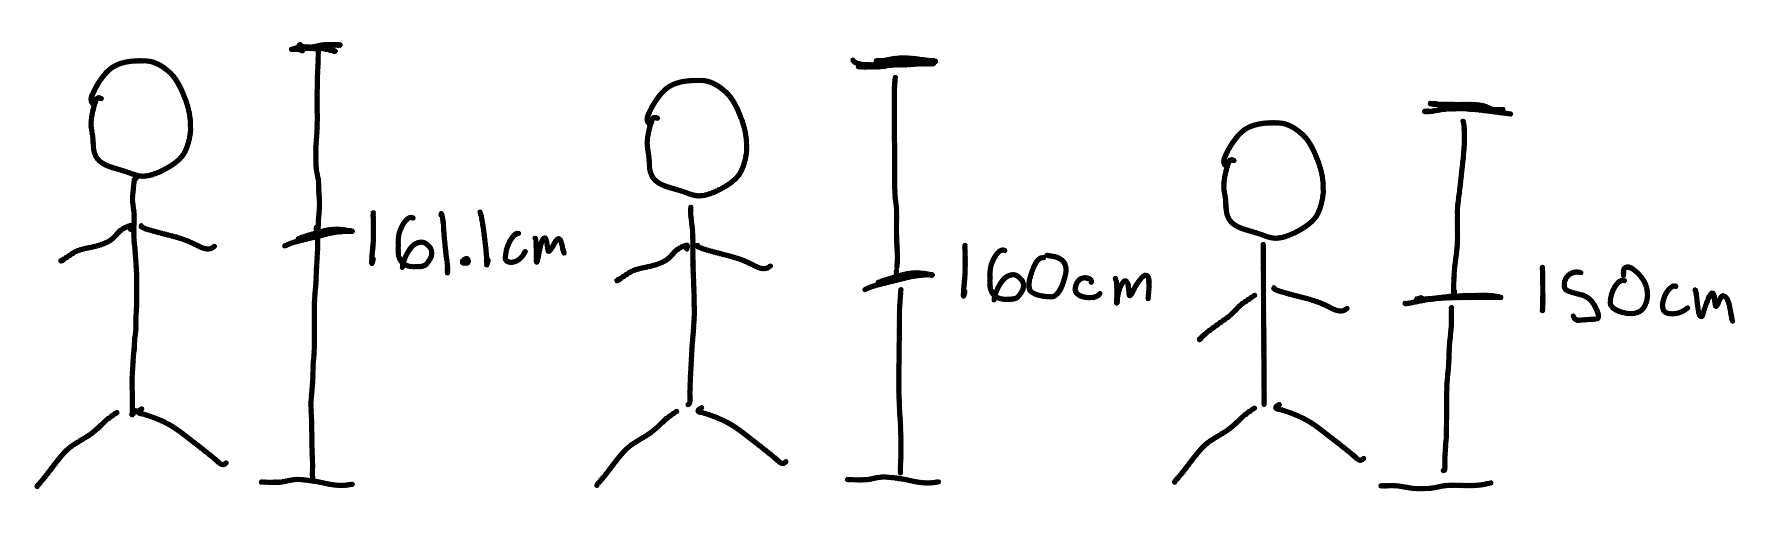
\includegraphics[width=5.0cm]{height.jpg}
        \caption{Height: Continuous Values}
      \end{figure}
    \end{column}
  \end{columns}
\end{frame}
\section{What is a moment?}
\begin{frame}{What is a moment?}
  \begin{itemize}
  \item Moments are confusing
  \item We know about a moment: The moment of inertia
  \item Maybe this will help?
  \end{itemize}
\end{frame}
\begin{frame}{Back to mass}
  \begin{itemize}
  \item How do we find the mass of something? \pause
    \begin{equation}
      m = \int\dd{m} = \int \rho\dd{V}
    \end{equation}\pause
  \item Something close to moment of inertia, center of mass: \pause
    \begin{equation}
      R_{cm} = \int r\dd{m} = \int r\rho\dd{V}
    \end{equation}\pause
  \item The moment of inertia is:\pause
    \begin{equation}
      I = \int r^2\dd{m} = \int r^2\rho\dd{V}
    \end{equation}
  \end{itemize}
\end{frame}
\begin{frame}{Takeaways}
  \begin{itemize}
  \item Power of '$r$' increases with each quantity
  \item Each one is a moment of mass
  \item First 'moment' = average
  \item Second 'moment' = how the mass is distributed
  \end{itemize}
\end{frame}
\begin{frame}{General moment of a distribution}
  \begin{itemize}
  \item A general $n^{\text{th}}$ moment of a distribution can be defined:
    \begin{equation}
      \mu_n=\int X^n\rho(X)\dd{X}
    \end{equation}
  \item Notice, this is the average of a function $X^n$ as opposed to just $X$ in the case of the 'average'
  \end{itemize}
\end{frame}
\begin{frame}{Characteristic Function}
  \begin{itemize}
  \item A characteristic function combines all of the moments at once, because of the power series expansion of the exponential in its definition:
    \begin{equation}
      \varphi_X(t)=\int\exp{iXt}\rho(X)\dd{X}
    \end{equation}
  \item This looks an awful lot like the Fourier transform of the probability density $\rho$, not sure of the implication of this.
  \end{itemize}
\end{frame}

\section{Cumulants}
\begin{frame}{An Alternative to Moments?}
  \begin{itemize}
  \item Take the log of characteristic function
  \item This way we directly get all of the moments:
    \begin{equation}
      K=\log\qty[\int\exp{tX}\rho(X)\dd{X}]
    \end{equation}
  \item Using the series expansion:
    \begin{equation}
      K(t)=\sum_{n=1}^\infty\kappa_n\frac{t^n}{n!}
    \end{equation}
  \item Where $\kappa_n$ is the $n^\text{th}$ moment!
  \end{itemize}
\end{frame}
\begin{frame}{What do these mean?}
  \begin{itemize}
  \item The $n^\text{th}$ cumulant can be calculated by taking the $n^\text{th}$ derivative of the generating function $K$ and evaluating at $t=0$
  \item Expanding the $\log$ gives an idea of how each of the moments relates to the corresponding cumulant
  \item The first four cumulants are as follows:
    \begin{enumerate}
    \item The mean/expectation value: Where is the data centered?
    \item Variance: How spread out is the data?
    \item Skewness: Does the data favor one end?
    \item Kurtosis: How much do the tails contribute compared to the center
    \end{enumerate}
  \end{itemize}
\end{frame}

\section{Binomial Distribution}
\begin{frame}{What is a Binomial Distribution?}
  \begin{itemize}
  \item Perform $n$ actions each with a yes or no answer
  \item Probability of yes $\equiv p$
  \item Probability of no $\equiv q$ 
  \end{itemize}
\end{frame}
\begin{frame}{Properties of a Binomial Distribution}
  \begin{itemize}
  \item Probability mass function, aka the probability of $k$ successes
    \begin{equation*}
      P(X=k)=\frac{n!}{k!(n-k)!}p^kq^{n-k}
    \end{equation*}
  \item Expected value
    \begin{equation*}
      E[X]=\mu=np
    \end{equation*}
  \item Variance (Second Moment)
    \begin{equation*}
      Var(X)=\sigma^2=npq=np(1-p)
    \end{equation*}
  \item Median
    \begin{equation*}
      \lfloor np\rfloor\quad\text{or}\quad\lceil np\rceil
    \end{equation*}
  \item Parameter $p$ is a number between $0,1$ inclusive
  \end{itemize}
\end{frame}
\begin{frame}{Examples}
  \begin{itemize}
  \item A certain percent of all emails are spam, if I receive $n$ emails in a day, what is the chance I get $k$ spam emails?
  \item Rolling a 20 on a 20-sided die in D\&D is really good, if I roll one $n$ times, what are the chances I get $k$ 20s?
  \item A special chicken can lay brown or white eggs, and brown eggs are really popular and sell well, so I want a lot of them, if this chicken lays $n$ eggs, what is the probability I get $k$ brown eggs?
  \end{itemize}
\end{frame}
\section{Poisson Distribution}
\begin{frame}{What is a Poisson Distribution?}
  \begin{itemize}
  \item You know an event has probability $\lambda$ of happening
  \item What is the probability of $n$ events in a time frame?
  \end{itemize}
\end{frame}
\begin{frame}{Properties of a Poisson Distribution}
    \begin{itemize}
  \item Probability mass function, aka the probability of $k$ events
    \begin{equation*}
      P(X=k)=\frac{\lambda^k}{k!}e^{-\lambda}
    \end{equation*}
  \item Expected value
    \begin{equation*}
      E[X]=\mu=\lambda
    \end{equation*}
  \item Variance (Second Moment)
    \begin{equation*}
      Var(X)=\sigma^2=\lambda
    \end{equation*}
  \item Parameter $\lambda$ can be any number greater than $0$
  \end{itemize}
\end{frame}
\begin{frame}{Examples}
  \begin{itemize}
  \item A poker player wins about $\lambda$ hands per hour, what are the chances of the player winning $k$ hands in a day?
  \item A website has found they get $\lambda$ visitors in a day on average, what is the probability of more than $k$ visitors in a day?
  \item My wifi sucks, on average it cuts out $\lambda$ times in a day on average, what is the probability I get $k$ in an hour when I have an assignment due?
  \end{itemize}
\end{frame}
\section{Normal Distribution}
\begin{frame}{What is a Normal Distribution?}
  \begin{itemize}
  \item The 'bell curve' distribution
  \item When we have large amounts of continuous data, it will usually follow a normal distribution
  \end{itemize}
\end{frame}
\begin{frame}{Properties of a Normal Distribution}
  \begin{itemize}
  \item Probability Density function:
    \begin{equation*}
      \rho(x)=\frac{1}{\sigma\sqrt{2\pi}}
      \exp{-\frac12\qty(\frac{x-\mu}\sigma)^2}
    \end{equation*}
  \item Mean and standard deviation are inputs:
    \begin{gather*}
      E[x]= \mu\\
      \mathrm{Var}(x)=\sigma^2
    \end{gather*}
  \item Mean, median, and mode are all $\mu$
  \item Parameter $\mu$ can be any real number
  \item Parameter $\sigma$ can be any real number besides $0$
  \end{itemize}
\end{frame}
\begin{frame}{More Properties}
  \begin{itemize}
  \item Bell shaped (Gaussian)
  \item Symmetric about $\mu$
  \item Almost all of the data is within $3\sigma$ of the mean
  \item The mode is unique, since a gaussian has a single peak
  \end{itemize}
\end{frame}
\begin{frame}{Examples}
  \begin{itemize}
  \item Standardized test scores with mean $\mu$ and variance $\sigma^2$
  \item The weight at birth of newborn babies 
  \item The probability density for the ground state of a quantum harmonic oscillator
  \item Poisson and Binomial distributions extended to continuous rather than discrete variables approximate a normal distribution
  \end{itemize}
\end{frame}
\end{document}